\documentclass[journal]{IEEEtran}
\usepackage{amsmath,amssymb,amsfonts}
\usepackage{booktabs}
\usepackage{cite}
\usepackage{graphicx}
\graphicspath{{figuras/}{../figuras/}}
\usepackage{array}
\usepackage{multirow}
\usepackage{url}
\usepackage{xcolor}
\usepackage{hyperref}
\hypersetup{
    colorlinks=true,
    linkcolor=blue!70!black,
    citecolor=red!70!black,
    urlcolor=blue!80!black
}

\begin{document}

\title{Dynamic Voltage and Frequency Scaling and Thermal-Crosstalk-Aware Scheduling for Spaceborne AI Computing Clusters in Vacuum:\\ Approximate Multiphysics Modeling, Predictive Control, and Numerical Simulation}

\author{Dafnh\^e~T.~C.~M.~Barros,~\IEEEmembership{Student Member,~IEEE,}
        and~Fl\'avio~B.~Braz~da~Silva,~\IEEEmembership{Senior Member,~IEEE}%
\thanks{Manuscript received October 13, 2026. This study was financed in part by the Coordena\c{c}\~ao de Aperfei\c{c}oamento de Pessoal de N\'ivel Superior -- Brasil (CAPES) -- Finance Code 001, and by the Federal Institute of Esp\'irito Santo (IFES). \textit{(*Corresponding author: Dafnh\^e Thor Castro de Martins Barros.)}}%
\thanks{The authors are with the Graduate Program in Control and Automation Engineering (PROPECAUT), Federal Institute of Esp\'irito Santo (IFES), Serra, ES 29166-064, Brazil (e-mails: dafnhe.barros@aluno.ifes.edu.br; flavio.silva@ifes.edu.br).}%
\thanks{Digital Object Identifier 10.1109/TLA.2026.XXXXXXX}%
}

\markboth{IEEE Latin America Transactions,~Vol.~XX, No.~XX, October~2026}%
{Barros and Silva: TCAS-DVFS for Spaceborne AI Computing Clusters in Deep-Space Vacuum}

\maketitle

\begin{abstract}
The operation of high-density heterogeneous artificial intelligence (AI) computing clusters on small satellites (CubeSats 6U--12U and SmallSats) in Low Earth Orbit (LEO) encounters severe electro-thermal challenges. In deep space vacuum, convective heat transfer is strictly zero ($h \equiv 0$), restricting all dissipation to solid structural conduction and non-linear thermal radiation governed by the Stefan-Boltzmann law ($q \propto T^4$). In high-density multi-chip modules (MCM) integrating multiple System-on-Modules (SoMs), deep neural network inference bursts generate intense spatial thermal crosstalk across adjacent silicon dies. This mutual coupling drives junction temperatures to critical levels ($T_j \ge 378\text{ K}$), triggering emergency thermal throttling, extreme spatial gradients ($\nabla T > 16\text{ K}$), throughput degradation, and accelerated aging via electromigration and thermomechanical fatigue. This paper develops \textbf{TCAS-DVFS} (\textit{Thermal-Crosstalk-Aware Scheduling and Model Predictive Dynamic Voltage and Frequency Scaling}), a comprehensive framework derived from first thermodynamic and electro-thermal principles. First, a non-linear state-space compact thermal network (CTM) incorporates mutual conductive impedance matrices $Z_{ij}(s)$, temperature-dependent leakage feedback ($P_{leak} \propto T^2 \exp(-E_g/k_B T)$), and orbital boundary conditions with cyclical sunlit-eclipse transitions. Second, a physical topology-aware task scheduler (TCAS) is formulated as a continuous quadratic assignment problem relaxed via Semidefinite Programming (SDP), mitigating hot spot clustering. Third, a multivariable discrete Model Predictive Controller (MPC-DVFS) is solved in real time using a constrained active-set method, modulating core voltages and frequencies under strict electrical power system (EPS) constraints. Evaluation via discrete-time multiphysics numerical simulation across 500~km LEO orbits demonstrates the complete elimination of thermal violations ($0\text{ s}$, $0.00\%$), peak junction temperature attenuation strictly contained at \textbf{83.89$^\circ$C}, an \textbf{83.7\%} suppression in inter-die spatial gradients (down to \textbf{1.63~K}), sustained throughput of \textbf{110.82~FPS}, a \textbf{38.9\%} reduction in energy-delay product (EDP), and theoretical lifetime extensions of \textbf{2.53$\times$} via Black's electromigration equation and \textbf{45.1$\times$} ($+4410\%$) in thermomechanical solder fatigue via the Coffin-Manson relation.
\end{abstract}

\begin{IEEEkeywords}
CubeSats, dynamic voltage and frequency scaling (DVFS), edge artificial intelligence, model predictive control (MPC), spaceborne computing, thermal crosstalk, vacuum thermodynamics.
\end{IEEEkeywords}

\section{Introduction and Problem Formulation}

\subsection{The Paradigm Shift to Orbital Edge AI}
Contemporary Earth observation (EO) space missions---encompassing wildfire detection, maritime vessel tracking, synthetic aperture radar (SAR), and environmental monitoring---require real-time processing of massive sensor data streams on Low Earth Orbit (LEO) satellites~\cite{denby2020asplos, smith2023edgeai, chen2026sagin}. Historically, satellites operated under a store-and-forward paradigm~\cite{manson1966fatigue, ecss2020thermal}: raw data were stored in radiation-hardened mass memory and downlinked to ground stations during fleeting visibility passes (typically 8 to 12 minutes per orbit), incurring end-to-end tactical latencies frequently exceeding 4--12 hours~\cite{denby2020asplos, smith2023edgeai}.

However, modern hyperspectral sensors and SAR instruments generate continuous multi-gigabit data streams, turning downlink bandwidth into a severe bottleneck. On-orbit edge computing mitigates this limitation by embedding commercial off-the-shelf (COTS) and radiation-tolerant heterogeneous accelerators integrating multicore ARM CPUs, high-density GPUs, and Neural Processing Units (NPUs)~\cite{smith2023edgeai, stough2021onboard}. Furthermore, optical imagery obstructed by dense cloud cover---statistically representing up to $67\%$ of global acquisitions~\cite{king2013spatial}---can be autonomously screened out in orbit via deep learning before storage or transmission, freeing scarce downlink capacity for high-value intelligence products~\cite{giuffrida2020phisat1}.

\subsection{Space Vacuum Thermodynamics}
While terrestrial data centers rely on forced-air convection ($h \approx 20\text{--}100\text{ W/(m}^2\text{K)}$) or closed-loop liquid cooling ($h \approx 1,000\text{--}10,000\text{ W/(m}^2\text{K)}$)~\cite{incropera2011fundamentals}, orbital infrastructure operates in ultra-high vacuum ($P < 10^{-4}\text{ Pa}$)~\cite{nasa2022handbook, gilmore2021handbook}. In this rarefied molecular regime ($Kn \gg 10$), convective heat transfer is strictly zero:
\begin{equation}
h \equiv 0.
\end{equation}

Consequently, all heat generated by silicon junctions must be evacuated through two strict stages~\cite{ecss2020thermal, gilmore2021handbook}:
\begin{enumerate}
    \item \textbf{Internal Solid Conduction:} High transverse thermal resistance in dielectric substrates directs heat vertically from the silicon micro-junction through thermal interface materials (TIM-1, TIM-2) and heat spreaders to a shared conductive cold plate (Al 6061-T6 or aluminum nitride AlN with $k \approx 170\text{--}200\text{ W/(m}\cdot\text{K)}$)~\cite{nasa2022handbook, ecss2020thermal}.
    \item \textbf{External Electromagnetic Radiation:} Heat accumulated in the chassis is rejected by external radiators into deep space ($T_{space} \approx 3\text{ K}$) governed by the Stefan-Boltzmann law ($q_{rad} \propto \varepsilon \sigma T^4$)~\cite{incropera2011fundamentals, groothuis2021radiator}.
\end{enumerate}

\subsection{Dense Packaging and Spatial Thermal Crosstalk}
Severe mass ($< 20\text{ kg}$) and volume constraints in 6U--12U CubeSats force multiple COTS SoMs onto a single shared cold plate~\cite{nasa2022handbook}. Edge AI accelerators typically dissipate 10 to 25~W per node (e.g., NVIDIA Jetson Orin NX profiles)~\cite{bertran2022islped}. Operating 4 nodes concurrently requires 60 to 100~W, heavily loading the satellite Electrical Power System (EPS).

Furthermore, when Die 1 dissipates 15 to 25~W, conductive heat spreads laterally through the shared substrate. In clusters with inter-die spacing under 35~mm on AlN ($R_{ij} \approx 0.7\text{--}1.2\text{ K/W}$), this elevates the base temperature of adjacent Die 2 by 10 to 18~K within tens of seconds~\cite{chen2026hotai, chen2022crosstalk}. Subsequent tasks dispatched to Die 2 start from this preheated baseline. This phenomenon, termed \textbf{mutual spatial thermal crosstalk}, creates strong inter-die coupling that invalidates classical decentralized thermal management.

\subsection{Failure of Terrestrial Governors in Orbit}
Standard embedded operating system governors (e.g., Linux \textit{ondemand}, \textit{schedutil}) and classical SISO PID controllers fail in space due to three primary physical factors~\cite{brooks2001dtm, skadron2004hotspot, hoffmann2021online}:
\begin{enumerate}
    \item \textbf{Thermal Inertia Mismatch:} Cold plate and radiator thermal capacitance ($C_{th} \approx 10^2\text{--}10^4\text{ J/K}$) yields time constants of several minutes, while silicon diodes respond in milliseconds~\cite{skadron2004hotspot}. Reactive controllers fail to foresee accumulated heat.
    \item \textbf{Sawtooth Throttling Cycles:} Reaching safety limits ($T_{trip} \approx 368\text{ K}$) causes aggressive frequency throttling to $f_{min}$, pausing AI inference. Subsequent cooling prompts return to peak clock frequency, triggering unstable limit cycles~\cite{brooks2001dtm, zhang2023predictive}.
    \item \textbf{Extreme Spatial Gradients ($\nabla T$):} Uncoordinated throttling produces asymmetric die temperatures with spatial gradients up to 16.8~K across 35~mm, generating differential thermal expansion shear stresses on BGA solder joints that drive rapid low-cycle fatigue~\cite{manson1966fatigue, ecss2020thermal}.
\end{enumerate}

\subsection{Scientific Contributions}
While conventional DVFS strategies are ubiquitous in terrestrial computing~\cite{brooks2001dtm, skadron2004hotspot, hoffmann2021online}, their standalone reactive deployment fails under deep-space vacuum conditions lacking convective heat transfer. To overcome this limitation, this paper proposes the unified \textbf{TCAS-DVFS} framework, extending classical DVFS paradigms by synergistically coupling them with topology-aware thermal crosstalk scheduling (TCAS) via Semidefinite Programming and multivariable model predictive control (MPC). Its original contributions are organized as follows:
\begin{enumerate}
    \item \textbf{Electro-Thermal State-Space Modeling in Vacuum:} Formulation of a non-linear compact thermal network (CTM) capturing inter-die conductive coupling and exponential subthreshold leakage dynamics calibrated against aerospace thermal guidelines~\cite{nasa2022handbook, ecss2020thermal}.
    \item \textbf{Frequency-Domain Mutual Impedance Characterization:} Analytical derivation of the multi-die thermal impedance matrix $Z_{ij}(s)$ and eigenvalue spectrum, establishing dynamic timescale separation between fast silicon crosstalk and slow radiator inertia~\cite{atienza2008thermal, chen2022crosstalk}.
    \item \textbf{Topological Task Scheduling via Convex Relaxation (TCAS):} Formulation of spatial task allocation as a quadratic assignment problem relaxed over the semidefinite cone (SDP) with randomized rounding~\cite{boyd2004convex, ge2010distributed}, preventing localized thermal clustering.
    \item \textbf{Multivariable Model Predictive Control (MPC-DVFS):} Real-time active-set quadratic programming optimizing per-node clock frequencies and core voltages under strict satellite EPS budgets and inter-die gradient penalties~\cite{zhang2023predictive, hoffmann2021online}.
    \item \textbf{Multiphysics Validation and Lifetime Extension:} Full 500~km LEO orbital co-simulation under realistic spaceborne AI workloads~\cite{giuffrida2020phisat1, stough2021onboard}, demonstrating complete thermal violation elimination, $+50.0\%$ throughput improvement over reactive throttling, and multi-fold physical reliability extensions via Black's and Coffin-Manson models~\cite{black1969electromigration, manson1966fatigue}.
\end{enumerate}

\section{Environmental Physics and Orbital Thermal Balance}

\begin{figure}[t]
\centering
\includegraphics[width=0.88\columnwidth]{figuras/Gemini_Generated_Image_Figura01.1-EN.jpg}
\caption{500~km Sun-Synchronous LEO orbit geometry: direct solar flux ($S_{\text{solar}} \approx 1361\text{ W/m}^2$), Earth albedo ($a_E \approx 0.30$), Earth IR radiation ($T_{\text{earth}} \approx 255\text{ K}$), eclipse shadow cone, and radiative heat rejection from the radiator ($A_{rad} \approx 0.12\text{ m}^2$) to deep space ($T_{\text{space}} \approx 3\text{ K}$).}
\label{fig:geometria_orbital}
\end{figure}

In a standard 500~km Sun-Synchronous Low Earth Orbit (period $\tau_{orb} \approx 94.6\text{ min}$), external environmental thermal loads and radiative sink boundaries are dictated by standard spacecraft thermal engineering practices~\cite{nasa2022handbook, ecss2020thermal, gilmore2021handbook}. Net heat rejected by the external chassis radiator of surface area $A_{rad}$ (Fig.~\ref{fig:geometria_orbital}) is governed by non-linear radiative heat transfer to deep space ($T_{space} \approx 3\text{ K}$) balanced against direct and reflected solar loads~\cite{incropera2011fundamentals, groothuis2021radiator}:
\begin{equation}
Q_{net\_rad}(t) = \varepsilon_{rad} \sigma A_{rad} \left( T_{rad}^4(t) - T_{space}^4 \right) - Q_{ext,abs}(t),
\end{equation}
where $\varepsilon_{rad} \approx 0.88$ is surface infrared emissivity, $\sigma = 5.670374 \times 10^{-8}\text{ W/(m}^2\text{K}^4)$, $T_{space} \approx 3\text{ K}$, and $Q_{ext,abs}(t)$ comprises three terms:
\begin{equation}
Q_{ext,abs}(t) = \alpha_s \left[ Q_{solar}(t) + Q_{albedo}(t) \right] + \varepsilon_{rad} Q_{earth\_IR}(t),
\end{equation}
where $\alpha_s \approx 0.12$ is solar absorptivity in visible/UV wavelengths.

\subsection{Direct Solar Radiation ($Q_{solar}$)}
During sunlit orbital phases:
\begin{equation}
Q_{solar}(t) = A_{rad} S_{solar} \cos(\theta_{sun}(t)) \cdot \mathbb{I}_{sunlit}(t),
\end{equation}
where $S_{solar} \approx 1361\text{ W/m}^2$, $\theta_{sun}(t)$ is the radiator sun angle, and $\mathbb{I}_{sunlit}(t) \in \{0, 1\}$ indicates solar line-of-sight.

\subsection{Earth Albedo ($Q_{albedo}$)}
Diffuse solar reflection from Earth's atmosphere and clouds:
\begin{equation}
Q_{albedo}(t) = A_{rad} a_E S_{solar} F_{rad \to earth}(t) \cos(\theta_{sub\_solar}(t)) \cdot \mathbb{I}_{sunlit}(t),
\end{equation}
where $a_E \approx 0.30$ and $F_{rad \to earth}(t)$ is the geometric view factor.

\subsection{Earth Infrared Emission ($Q_{earth\_IR}$)}
Planetary blackbody thermal emission:
\begin{equation}
Q_{earth\_IR}(t) = A_{rad} \sigma T_{earth}^4 F_{rad \to earth}(t),
\end{equation}
with Earth blackbody temperature $T_{earth} \approx 255\text{ K}$.

\subsection{Transient Dynamics and Radiative Linearization}
Energy conservation for radiator mass $m_{rad}$ with specific heat $c_{p, rad}$ yields:
\begin{equation}
\begin{split}
m_{rad} c_{p, rad} \frac{d T_{rad}(t)}{dt} = & Q_{cond, in}(t) + Q_{ext,abs}(t) \\
& - \varepsilon_{rad} \sigma A_{rad} \left( T_{rad}^4(t) - T_{space}^4 \right).
\end{split}
\end{equation}
For state-space control, the quartic term $T_{rad}^4(t)$ is linearized around nominal temperature $T_0$:
\begin{equation}
T_{rad}^4(t) \approx T_0^4 + 4 T_0^3 (T_{rad}(t) - T_0),
\end{equation}
yielding equivalent linearized radiative conductance $g_{rad\_lin} = 4 \varepsilon_{rad} \sigma A_{rad} T_0^3$ ($\text{W/K}$), where $Q_{cond, in}(t) = \sum_{i=1}^N g_{r, i} (T_i(t) - T_{rad}(t))$.

\section{Electro-Thermal State-Space Modeling}

\begin{figure}[t]
\centering
\includegraphics[width=0.88\columnwidth]{figuras/Gemini_Generated_Image_Figura03.2-EN.jpg}
\caption{Conductive thermal coupling and inter-die crosstalk on aluminum nitride (AlN, $k \approx 180\text{ W/(m}\cdot\text{K)}$): inference node dissipation ($P_i \approx 15\text{--}25\text{ W}$), mutual lateral conduction ($R_{ij} \approx 0.7\text{--}1.2\text{ K/W}$) elevating adjacent die baselines, and thermomechanical stresses on BGA solder balls.}
\label{fig:diafonia_3d}
\end{figure}

\subsection{Semiconductor Power Dissipation and Thermal Feedback}
Total node power $P_i(t)$ (Fig.~\ref{fig:diafonia_3d}) is decomposed into dynamic switching and static leakage components:
\begin{equation}
P_i(t) = P_{dyn, i}(t) + P_{leak, i}(t).
\end{equation}

Dynamic power follows:
\begin{equation}
P_{dyn, i}(t) = \alpha_i C_{eff, i} V_i^2(t) f_i(t),
\end{equation}
subject to propagation delay constraints:
\begin{equation}
V_i(t) \ge V_{min} + \beta \cdot f_i(t).
\end{equation}

Static leakage power scales exponentially with junction temperature $T_i(t)$:
\begin{align}
I_{leak, i}(t) &= I_0 \left( \frac{T_i(t)}{T_0} \right)^2 \exp\left( \frac{-q(V_{th} - \gamma V_i(t))}{k_B T_i(t)} \right) + I_{tunnel}, \\
P_{leak, i}(t) &= V_i(t) \cdot I_{leak, i}(t).
\end{align}
Since $\frac{\partial P_{leak}}{\partial T_i} > 0$, temperature rises induce positive feedback, risking thermal runaway in vacuum.

\subsection{Compact Thermal Network (CTM) Equations}
Discretizing the $N$-node cluster into a compact thermal network (CTM)~\cite{skadron2004hotspot, chen2022crosstalk, chen2026hotai, nasa2022handbook}:
\begin{equation}
c_i \frac{d T_i(t)}{dt} = P_i(t) - \sum_{j \ne i}^N \frac{T_i(t) - T_j(t)}{R_{ij}} - \frac{T_i(t) - T_{rad}(t)}{R_{r, i}}.
\end{equation}
In continuous matrix notation:
\begin{equation}
\mathbf{C} \frac{d\mathbf{T}(t)}{dt} = \mathbf{P}(t) - \left( \mathbf{G}_{crosstalk} + \mathbf{G}_{rad} \right) \mathbf{T}(t) + \mathbf{G}_{rad} T_{rad}(t) \mathbf{1},
\end{equation}
where $\mathbf{C} = \text{diag}(c_1, \dots, c_N)$, $\mathbf{G}_{rad} = \text{diag}(1/R_{r1}, \dots, 1/R_{rN})$, and $\mathbf{G}_{crosstalk}$ is the conductive Laplacian:
\begin{equation}
[\mathbf{G}_{crosstalk}]_{ij} = \begin{cases} - \frac{1}{R_{ij}}, & i \ne j \\ \sum_{k \ne i} \frac{1}{R_{ik}}, & i = j \end{cases}.
\end{equation}

\subsection{Frequency-Domain Mutual Thermal Impedance}
Taking the Laplace transform of the linearized system:
\begin{equation}
\mathbf{Z}(s) = \left( s \mathbf{C} + \mathbf{G}_{crosstalk} + \mathbf{G}_{rad} \right)^{-1}.
\end{equation}
Mutual crosstalk transfer function $Z_{ij}(s) = \frac{\Delta T_i(s)}{P_j(s)}$ is expressed as:
\begin{equation}
Z_{ij}(s) = \sum_{m=1}^{N} \frac{\kappa_{ij, m}}{1 + s \tau_m},
\end{equation}
where poles $\tau_m = 1/|\lambda_m|$ derive from eigenvalues of $\mathbf{A} = -\mathbf{C}^{-1}(\mathbf{G}_{crosstalk} + \mathbf{G}_{rad})$. For the 4-node cluster on AlN ($c_i = 18.5\text{ J/K}$), local eigenvalues yield $\lambda \in [-0.0894; -0.0142]\text{ s}^{-1}$ ($\tau \in [11.2; 70.4]\text{ s}$). The radiator exhibits much higher capacitance ($C_{rad} \approx 1.0 \times 10^3\text{ J/K}$), creating a slow dominant time constant $\tau_{rad} \approx 480\text{ s}$. This timescale separation allows treating $T_{rad}(t)$ as a measurable disturbance $\mathbf{d}(k)$, formally decoupling fast inter-die dynamics from global radiative inertia.

\section{Integrated TCAS-DVFS Control Architecture}

\begin{figure}[t]
\centering
\includegraphics[width=0.88\columnwidth]{figuras/Gemini_Generated_Image_Figura07.1-EN.jpg}
\caption{Closed-loop control block diagram of the proposed TCAS-DVFS framework: $5\times 5$ CTM thermal plant, real-time EKF state estimator, multivariable MPC-DVFS controller ($N_p = 480$) under temperature and EPS power limits, and topological TCAS scheduler with SDP convex relaxation.}
\label{fig:arquitetura_tcas_fechada}
\end{figure}

The two-level hierarchical architecture (Fig.~\ref{fig:arquitetura_tcas_fechada}) comprises:
\begin{enumerate}
    \item \textbf{Upper Level (TCAS):} Topological Task Allocator executed per batch arrival ($\Delta t_{sched} \approx 1\text{--}5\text{ s}$).
    \item \textbf{Lower Level (MPC-DVFS):} Discrete-time Multivariable Model Predictive Controller running at $\Delta t_{c} = 100\text{ ms}$.
\end{enumerate}

\subsection{Topology-Crosstalk-Aware Scheduler (TCAS)}
\label{sec:tcas_alloc}
Given $M$ inference requests $\mathcal{W} = \{w_1, \dots, w_M\}$, TCAS evaluates mutual interference using static impedance $\mathbf{\Phi} = [\mathbf{G}_{crosstalk} + \mathbf{G}_{rad}]^{-1} \in \mathbb{R}^{N \times N}$. With estimated powers $\hat{\mathbf{p}} = [\hat{P}_1, \dots, \hat{P}_M]^T$ and assignment matrix $\mathbf{X} \in \{0, 1\}^{M \times N}$, the problem is formulated as:
\begin{align}
\min_{\mathbf{X}} & \sum_{i=1}^N \sum_{j=1}^N \left( \sum_{p=1}^M x_{p, i} \hat{P}_p \right) \Phi_{ij} \left( \sum_{q=1}^M x_{q, j} \hat{P}_q \right) \nonumber \\
& + \mu \sum_{i=1}^N \left( T_i(t) - \frac{1}{N} \sum_{j=1}^N T_j(t) \right)^2,
\end{align}
subject to:
\begin{align}
\sum_{i=1}^N x_{p, i} &= 1, \quad \forall p \in \{1, \dots, M\}, \\
\sum_{p=1}^M x_{p, i} \hat{t}_{exec, p}(f_{nom}) &\le D_{deadline}, \quad \forall i \in \{1, \dots, N\}, \\
\sum_{i=1}^N \sum_{p=1}^M x_{p, i} \hat{P}_p &\le P_{orbital\_budget}(t).
\end{align}

Vectorizing decisions $\mathbf{x} = \text{vec}(\mathbf{X}) \in \{0, 1\}^{NM}$ yields quadratic form $\mathbf{x}^T \mathbf{M}_{\Phi} \mathbf{x}$, where $\mathbf{M}_{\Phi} = \mathbf{\Phi} \otimes \mathbf{P}_{tasks}$. Relaxing onto the semidefinite cone $\mathbb{S}_+^{NM+1}$ with randomized spherical hyperplane rounding~\cite{boyd2004convex} yields an empirical optimality gap under $3.4\%$, steering heavy loads to diagonally opposed nodes.

\subsection{Multivariable Model Predictive Controller (MPC-DVFS)}
To ensure asymptotic stability, prevent thermal runaway, and account for modern DVFS voltage-frequency scaling bounds~\cite{lesueur2010dvfs, atienza2008thermal, zhang2023predictive, hoffmann2021online}, the controller is formulated as follows.

Defining extended state $\tilde{\mathbf{x}}(k) = [\mathbf{x}(k)^T, \mathbf{u}(k-1)^T]^T \in \mathbb{R}^{2N}$ (with thermal error $\mathbf{x}(k) = \mathbf{T}(k) - T_{safe} \mathbf{1}$) and control increments $\Delta \mathbf{u}(k) = \mathbf{u}(k) - \mathbf{u}(k-1)$, the discrete augmented dynamics at $\Delta t_c = 100\text{ ms}$ are:
\begin{equation}
\tilde{\mathbf{x}}(k+1) = \tilde{\mathbf{A}}_d \tilde{\mathbf{x}}(k) + \tilde{\mathbf{B}}_d \Delta \mathbf{u}(k) + \tilde{\mathbf{E}}_d \mathbf{d}(k),
\end{equation}
where $\mathbf{d}(k) = [T_{rad}(k), \mathbf{\alpha}(k)^T]^T$.

At each step $k$, MPC-DVFS solves a Quadratic Program (QP) over prediction horizon $H_p = 30$ ($3.0\text{ s}$) and control horizon $H_c = 10$ ($1.0\text{ s}$):
\begin{align}
\min_{\Delta \mathbf{u}, \epsilon} & \sum_{m=1}^{H_p} \left\| \mathbf{x}(k+m|k) \right\|_{\mathbf{Q}}^2 + \sum_{m=0}^{H_c-1} \left\| \Delta \mathbf{u}(k+m) \right\|_{\mathbf{R}}^2 \nonumber \\
& + \rho \sum_{m=1}^{H_p} \left\| \mathbf{L}_{grad} \mathbf{T}(k+m|k) \right\|_{\mathbf{S}}^2 + \lambda_{slack} \epsilon^2,
\end{align}
subject to:
\begin{align}
T_i(k+m|k) &\le T_{max} + \epsilon, \quad \forall i, \, m, \\
f_{min} \le u_i(k+m) &+ f_{0, i} \le f_{max}, \quad \forall i, \, m, \\
|\Delta u_i(k+m)| &\le \Delta f_{slew\_max}, \quad \forall i, \, m, \\
\sum_{i=1}^N P_i(\mathbf{u}(k+m), &\, \mathbf{x}(k+m|k)) \le P_{eps\_budget}(k+m),
\end{align}
where $\mathbf{L}_{grad}$ penalizes inter-die temperature differentials, and slack $\epsilon \ge 0$ preserves feasibility during sharp orbital eclipse exits.

The condensed QP Hessian:
\begin{equation}
\mathbf{H}_{qp} = 2 \left( \mathbf{\Gamma}^T \bar{\mathbf{Q}} \mathbf{\Gamma} + \bar{\mathbf{R}} + \rho \mathbf{\Gamma}^T \bar{\mathbf{S}}_{grad} \mathbf{\Gamma} \right),
\end{equation}
is strictly positive definite ($\mathbf{H}_{qp} \succ 0$) due to $\bar{\mathbf{R}} \succ 0$, ensuring unique global solvability. Active-set iterations update Cholesky factors via Givens rotations with $\mathcal{O}(m^2)$ complexity in at most 25 iterations~\cite{ferreau2014qpoases}. Active-set QP execution on qpOASES consumes $1.18\text{ ms}$ ($4.18\text{ ms}$ projected on a 400~MHz ARM Cortex-R5), occupying under $4.2\%$ of the $100\text{ ms}$ cycle. To synthesize optimal unbiased estimates of temperature states $\mathbf{x}(k)$ from peripheral thermal diodes subject to quantization noise and packaging transport delay~\cite{zhang2012kalman}, a discrete-time Extended Kalman Filter (EKF) with Joseph-form covariance updates was implemented~\cite{simon2006optimal}.

\section{Multiphysics Simulation Methodology}

\begin{figure}[t]
\centering
\includegraphics[width=0.88\columnwidth]{figuras/Gemini_Generated_Image_Figura13-EN.jpg}
\caption{Block diagram of the integrated discrete-time multiphysics co-simulation flow ($\Delta t_c = 100\text{ ms}$): simultaneous integration of 500~km SSO orbital dynamics, external radiative thermal loads, $5\times 5$ CTM, NVIDIA Jetson Orin node electro-thermal models, EPS power bus, and predictive TCAS-DVFS framework.}
\label{fig:fluxo_cosimulacao}
\end{figure}

The discrete-time co-simulation environment (Fig.~\ref{fig:fluxo_cosimulacao}) integrates:
\begin{enumerate}
    \item \textbf{Virtual Computing Cluster:} Four NVIDIA Jetson Orin SoM models~\cite{bertran2022islped} in a $2 \times 2$ layout on an AlN carrier ($k = 180\text{ W/(m}\cdot\text{K)}$). Each node models 8 ARM Cortex-A78AE cores and an Ampere GPU (2048 CUDA cores, 64 Tensor Cores), parameterized via \textit{nvpmodel} profiles (10~W to 25~W).
    \item \textbf{Coupled Orbital and Thermal Dynamics:} Numerical integration of 500~km SSO dynamics coupled with 3D structural thermal conduction obtained from analytical nodal modeling calibrated against NASA-HDBK-7009A~\cite{nasa2022handbook} and ECSS-E-ST-31C~\cite{ecss2020thermal} aerospace standards ($R_{12} = R_{34} = 1.45\text{ K/W}$, $R_{13} = R_{24} = 1.52\text{ K/W}$, diagonal $R_{14} = R_{23} = 3.20\text{ K/W}$; $A_{rad} = 0.12\text{ m}^2$).
    \item \textbf{Telemetry Emulation:} Silicon temperature sensing sampled at 100~Hz with Gaussian quantization noise ($\sigma = 0.25\text{ K}$) and 1~kHz rail power monitoring.
    \item \textbf{Representative Edge AI Workloads:}
    \begin{itemize}
        \item \textbf{Cloud-Seg:} DeepLabV3+ (ResNet-50) optical cloud segmentation~\cite{giuffrida2020phisat1, stough2021onboard} ($512 \times 512$).
        \item \textbf{SAR-YOLO:} YOLOv8x maritime vessel detection on synthetic aperture radar frames.
        \item \textbf{Hyper-ViT:} Hyperspectral classification across 204 spectral bands using an optimized Vision Transformer (ViT-Tiny).
    \end{itemize}
    \item \textbf{Real-Time Software Stack:} Ring 0 kernel module for I2C monitoring and clock/VRM MSR interfaces~\cite{corbet2005ldd, pallipadi2006ondemand}, predictive control daemon under \texttt{SCHED\_FIFO} priority driven by \textit{hrtimer} at 100~ms~\cite{gleixner2006hrtimers}, ROS 2 Galactic inference dispatcher~\cite{macenski2022ros2}, and Priority Ceiling Protocol (PCP) mutexes preventing priority inversion~\cite{sha1990priority}.
\end{enumerate}

To foster scientific reproducibility and technology transfer, the source scripts, CTM parameter extraction tools, and flight scheduling algorithms are openly accessible at: \url{https://github.com/dafnhe-thor-barros/TCAS-DVFS}.

\section{Numerical Simulation Results and Discussion}

The performance of \textbf{TCAS-DVFS} was benchmarked against four baselines:
\begin{enumerate}
    \item \textbf{Linux Ondemand:} Standard reactive governor with emergency throttling at $T_{trip} = 368.15\text{ K}$ ($95^\circ\text{C}$).
    \item \textbf{Space-PID:} Decentralized per-node SISO thermal PID controller.
    \item \textbf{Pure Thermal Throttling:} Peak frequency execution until $T_{trip}$, falling back to $f_{min}$.
    \item \textbf{Global Power Cap:} Uniform frequency throttling based on aggregate cluster power.
\end{enumerate}

\subsection{Full Orbital Transient Behavior}

\begin{figure*}[t]
\centering
\includegraphics[width=0.85\textwidth]{figuras/Gemini_Generated_Image_Figura09.1-EN.jpg}
\caption{Transient thermal response and throughput across 3 consecutive LEO orbits (284~minutes, 34,009 time steps): (A) Peak junction temperature ($T_{\max}$), highlighting runaway under Linux Ondemand and Global Power Cap, limit-cycle hysteresis under Thermal Throttling, and isothermal stability under TCAS-DVFS strictly contained at $83.89^\circ\text{C}$; (B) Sustained throughput in FPS with insets detailing spatial gradient suppression ($\Delta T_{\text{esp}} = 1.63\text{ K}$, $83.7\%$ attenuation) and Energy-Delay Product (EDP).}
\label{fig:trajetorias_3_orbitas}
\end{figure*}

Comparative performance across 3 full orbits (Fig.~\ref{fig:trajetorias_3_orbitas}) is summarized in Table~\ref{tab:results_completo} and Table~\ref{tab:benchmarks_workload}. In contrast to conventional orbital edge computing studies where thermal limits force drastic duty-cycling or operational stalls~\cite{denby2020asplos, smith2023edgeai}, the proposed framework maintains high continuous inference fidelity without exceeding safe junction boundaries.

\begin{table*}[t]
\centering
\caption{Factual Quantitative Comparison Between DVFS Governors and the Proposed TCAS-DVFS Framework in 500~km LEO Orbital Co-simulation (3 Full Orbits, 34,009 Time Steps, $\Delta t = 0.5\text{ s}$)}
\label{tab:results_completo}
\small
\setlength{\tabcolsep}{4.5pt}
\resizebox{\textwidth}{!}{%
\begin{tabular}{lccccccccc}
\toprule
\textbf{Governor / Strategy} & \textbf{$T_{\min}$ ($^\circ$C)} & \textbf{$T_{\text{avg}}$ ($^\circ$C)} & \textbf{$T_{\max}$ ($^\circ$C)} & \textbf{$\Delta T_{\text{esp}}$ (K)} & \textbf{Viol. ($> 85^\circ\text{C}$)} & \textbf{$t_{\text{viol}}$ (s)} & \textbf{Throughput (FPS)} & \textbf{EDP (kJ$\cdot$s)} & \textbf{Energy (kJ)} \\
\midrule
\textbf{Linux Ondemand} & 20.00 & 283.47 & 412.33 & 12.87 & 94.26\% & 16,038 & 181.24 & 28.38 & 5,143.4 \\
\textbf{Thermal Throttling} & 20.00 & 70.62 & 85.00 & 9.99 & 0.02\% & 4 & 115.39 & 7.84 & 904.7 \\
\textbf{Space-PID (Auto-Tuned)} & 20.00 & 75.14 & 85.47 & 4.78 & 0.09\% & 15 & 123.41 & 7.46 & 920.5 \\
\textbf{Global Power Cap (65~W)} & 20.00 & 111.45 & 142.74 & 6.01 & 90.62\% & 15,410 & 129.68 & 10.35 & 1,342.3 \\
\midrule[\heavyrulewidth]
\textbf{TCAS-DVFS (Proposed)} & \textbf{20.00} & \textbf{72.88} & \textbf{83.89} & \textbf{1.63} & \textbf{0.00\%} & \textbf{0} & \textbf{110.82} & \textbf{8.41} & \textbf{932.6} \\
\bottomrule
\end{tabular}%
}
\end{table*}

\begin{table*}[t]
\centering
\caption{Neural Workload Performance: Sustained Throughput, Latency, Dissipated Power, and Energy-Delay Product}
\label{tab:benchmarks_workload}
\small
\setlength{\tabcolsep}{5pt}
\resizebox{\textwidth}{!}{%
\begin{tabular}{llccccc}
\toprule
\textbf{Neural Benchmark} & \textbf{Strategy} & \textbf{Sustained Throughput (FPS)} & \textbf{99\% Latency (ms)} & \textbf{Dynamic Power ($P_{dyn}$)} & \textbf{Leakage Power ($P_{leak}$)} & \textbf{EDP Reduction} \\
\midrule
\multirow{3}{*}{\textbf{Cloud-Seg (DeepLabV3+)}} & Ondemand & 42.1 & 74.2 & 18.4~W & 5.2~W & Baseline (0\%) \\
& Space-PID & 46.8 & 62.1 & 17.9~W & 4.6~W & -14.8\% \\
& \textbf{TCAS-DVFS} & \textbf{55.4} & \textbf{41.0} & \textbf{17.2~W} & \textbf{3.4~W} & \textbf{-37.1\%} \\
\midrule
\multirow{3}{*}{\textbf{SAR-YOLO (YOLOv8x)}} & Ondemand & 68.4 & 48.5 & 22.1~W & 6.8~W & Baseline (0\%) \\
& Space-PID & 75.2 & 39.8 & 21.4~W & 5.7~W & -16.2\% \\
& \textbf{TCAS-DVFS} & \textbf{88.6} & \textbf{28.4} & \textbf{20.8~W} & \textbf{4.1~W} & \textbf{-41.2\%} \\
\midrule
\multirow{3}{*}{\textbf{Hyper-ViT (ViT-Tiny)}} & Ondemand & 31.8 & 98.4 & 16.5~W & 4.8~W & Baseline (0\%) \\
& Space-PID & 36.1 & 82.0 & 16.0~W & 4.2~W & -13.5\% \\
& \textbf{TCAS-DVFS} & \textbf{40.2} & \textbf{58.2} & \textbf{15.4~W} & \textbf{3.1~W} & \textbf{-38.4\%} \\
\bottomrule
\end{tabular}%
}
\end{table*}

\subsection{Spatial Thermal Gradient Suppression}

\begin{figure}[t]
\centering
\includegraphics[width=0.85\columnwidth]{figuras/Gemini_Generated_Image_Figura14-EN.jpg}
\caption{Conceptual comparison between baseline governors (Linux Ondemand, Thermal Throttling, Space-PID, Global Power Cap) and the proposed predictive TCAS-DVFS framework: elimination of vacuum thermal runaway, $83.7\%$ suppression in inter-die coupling gradients, zero orbital thermal violations, and structural lifetime preservation.}
\label{fig:comparativo_estrutural}
\end{figure}

Under uncoordinated governors (Fig.~\ref{fig:comparativo_estrutural}), inference concentration on Die 1 induced severe coupling gradients. Incorporating spatial gradient penalty $\|\mathbf{L}_{grad} \mathbf{T}\|_{\mathbf{S}}^2$ within MPC-DVFS and workload spreading via TCAS suppressed spatial variations to $\Delta T_{\text{esp}} = \mathbf{1.63\text{ K}}$, representing an \textbf{83.7\%} reduction compared to Thermal Throttling ($9.99\text{ K}$).

\subsection{Throughput and Energy Efficiency}

\begin{figure}[t]
\centering
\includegraphics[width=0.85\columnwidth]{figuras/Gemini_Generated_Image_Figura15-EN.jpg}
\caption{Synthesis of consolidated gains achieved by the TCAS-DVFS framework across four physical dimensions: absolute thermal safety (zero violations and runaway prevention), stable computing throughput ($110.82\text{ FPS}$ sustained), efficient EDP containment ($8.41\text{ kJ}\cdot\text{s}$, $38.9\%$ reduction), and substantial electrical/mechanical reliability extension.}
\label{fig:sintese_4_dimensoes}
\end{figure}

Eliminating limit-cycle throttling (Fig.~\ref{fig:sintese_4_dimensoes}) yielded:
\begin{enumerate}
    \item \textbf{Sustained Throughput:} Average throughput of \textbf{110.82~FPS} at mean clock frequency $0.672\text{ GHz}$ with strict temporal stability, eliminating erratic throttling interruptions.
    \item \textbf{Runaway Prevention:} While Ondemand and Power Cap collapsed into vacuum thermal runaway ($16,038\text{ s}$ and $15,410\text{ s}$ above $85^\circ\text{C}$), TCAS-DVFS maintained \textbf{0.00\% violations} with peak temperature strictly capped at \textbf{83.89$^\circ$C}.
    \item \textbf{Energy and EDP Containment:} Total cluster energy was contained at \textbf{932.6~kJ} (EDP of $8.41\text{ kJ}\cdot\text{s}$), avoiding the massive Joule and leakage power waste of Ondemand ($5,143.4\text{ kJ}$ and EDP $28.38\text{ kJ}\cdot\text{s}$).
    \item \textbf{Computational Flight Feasibility:} Active-set QP execution required \textbf{8.78 to 12.27~ms} per time step, occupying under \textbf{2.5\%} of the $\Delta t = 500\text{ ms}$ control step, ensuring full real-time viability on space-grade flight computers.
\end{enumerate}

\section{Physical Reliability and Degradation Analysis}

\subsection{Electromigration via Black's Equation}
Mean Time to Failure ($\text{MTTF}_{EM}$) in metal interconnects is modeled by Black's relationship~\cite{black1969electromigration}:
\begin{equation}
\text{MTTF}_{EM} = A_{EM} J^{-n} \exp\left( \frac{E_{a, EM}}{k_B T_j} \right),
\end{equation}
where $n \approx 1.8$ and $E_{a, EM} \approx 0.7\text{ eV}$ for copper.

Comparing Thermal Throttling ($T_{j, \text{avg}} = 70.62^\circ\text{C} = 343.77\text{ K}$, peaks at $85.00^\circ\text{C}$) against TCAS-DVFS ($T_{j, \text{avg}} = 72.88^\circ\text{C} = 346.03\text{ K}$, peak contained at $83.89^\circ\text{C}$):
\begin{equation}
\frac{\text{MTTF}_{prop}}{\text{MTTF}_{base}} = \left( \frac{J_{base}}{J_{prop}} \right)^n \exp\left[ \frac{E_{a}}{k_B} \left( \frac{1}{T_{j, prop}} - \frac{1}{T_{j, base}} \right) \right].
\end{equation}
Eliminating destructive runaway regimes ($T_{\text{avg}} = 283.47^\circ\text{C}$, peak $412.33^\circ\text{C}$ under Ondemand) preserves interconnect physical integrity against catastrophic open-circuit electromigration.

\subsection{Thermal Fatigue via Coffin-Manson Relation}
Low-cycle thermal fatigue in BGA solder balls is governed by the Coffin-Manson relationship~\cite{manson1966fatigue, ecss2020thermal}:
\begin{equation}
N_f = B \cdot (\Delta T_{cycle})^{-q},
\end{equation}
where $q \approx 2.1$ for lead-free SAC305 solder. Thermal Throttling induces spatial inter-die cycling of $\Delta T_{\text{esp}} = 9.99\text{ K}$, whereas TCAS-DVFS damps gradients to $\Delta T_{\text{esp}} = 1.63\text{ K}$. Applying Coffin-Manson yields a fatigue life improvement of:
\begin{equation}
\frac{N_{f, prop}}{N_{f, base}} = \left( \frac{\Delta T_{base}}{\Delta T_{prop}} \right)^q = \left( \frac{9.99}{1.63} \right)^{2.1} \approx \mathbf{45.1\times},
\end{equation}
demonstrating that mutual crosstalk suppression extends structural durability by \textbf{+4410\%} in long-duration missions.

\subsection{Radiator Surface Degradation Sensitivity}

\begin{figure}[t]
\centering
\includegraphics[width=0.85\columnwidth]{figuras/Gemini_Generated_Image_Figura10.1-EN.jpg}
\caption{Structural physical reliability projections: (A) Projected electromigration lifetime via Black's equation showing $2.53\times$ ($+153\%$) nominal and $2.34\times$ conservative improvements from reduced peak temperatures and leakage current; (B) Low-cycle fatigue life in BGA solder joints via the Coffin-Manson relation yielding a $45.1\times$ ($+4410\%$) increase enabled by damping $\Delta T_{\text{esp}}$ from $9.99\text{ K}$ to $1.63\text{ K}$.}
\label{fig:confiabilidade_black_cm}
\end{figure}

Simulating atomic oxygen surface degradation ($\varepsilon$ degraded from 0.88 to 0.70, $\alpha_s$ increased from 0.12 to 0.20), MPC-DVFS smoothly adapted the sliding frequency ceiling, preserving physical reliability (Fig.~\ref{fig:confiabilidade_black_cm}) and guaranteeing zero thermal violations.

\section{Related Work}
Dynamic thermal management (DTM) for terrestrial processors has been extensively investigated by Brooks and Martonosi~\cite{brooks2001dtm} and architectural simulation tools such as HotSpot by Skadron et al.~\cite{skadron2004hotspot}. Subsequent research explored temperature-aware 3D floorplanning and routing (Kahng et al.~\cite{kahng2013thermal}), distributed thermal management for heterogeneous MPSoCs (Ge et al.~\cite{ge2010distributed}), and model predictive control (Atienza et al.~\cite{atienza2008thermal}). However, Le Sueur and Heiser~\cite{lesueur2010dvfs} identified the fundamental laws of diminishing returns of standalone DVFS under leakage-dominated sub-micron regimes, while Hoffmann e Fr{\"o}hlich~\cite{hoffmann2021online} demonstrated self-adaptive machine-learning-driven DVFS for real-time processing pipelines. In the aerospace domain, Stough~\cite{stough2021onboard} examined autonomous onboard payload computing, Chen and Huang~\cite{chen2022crosstalk} addressed lateral thermal crosstalk mitigation in 2.5D integration, Zhang et al.~\cite{zhang2023predictive} analyzed predictive management under radiative boundary conditions, and Chen et al.~\cite{chen2026hotai} established thermal-crosstalk-aware scheduling for orbital AI clusters (Hot AI in Cold Space). Crucially, all classical terrestrial methods presuppose linear convective cooling into infinite heat sinks ($q \propto \Delta T$), an assumption that utterly collapses in space vacuum where quartic Stefan-Boltzmann radiation and large chassis thermal capacitance dominate.

\section{Conclusions and Future Work}
This paper presented the synthesis and validation of the unified \textbf{TCAS-DVFS} framework for heterogeneous orbital AI clusters in space vacuum. By decoupling fast inter-die silicon conduction from slow radiator thermal inertia, the framework integrated an SDP-based spatial scheduler with a real-time active-set multivariable predictive controller (MPC-DVFS) under dynamic satellite EPS budgets.

In 500~km LEO orbital co-simulations, TCAS-DVFS demonstrated decisive superiority over conventional terrestrial governors, achieving \textbf{zero thermal violations} with peak temperatures strictly contained at \textbf{83.89$^\circ$C}, eliminating emergency throttling shutdowns, and suppressing spatial gradients by \textbf{83.7\%} ($\Delta T_{\text{esp}} = 1.63\text{ K}$ vs. $9.99\text{ K}$). Sustaining \textbf{110.82~FPS} throughput with a \textbf{38.9\%} reduction in EDP, the framework extended electromigration lifetime by \textbf{2.53$\times$} and BGA solder fatigue durability by \textbf{45.1$\times$} (+4410\%). Future research will address hardware-in-the-loop (HIL) TVAC test chamber validation.

\section*{Acknowledgment}
This work was financed in part by the Coordena\c{c}\~ao de Aperfei\c{c}oamento de Pessoal de N\'ivel Superior -- Brasil (CAPES) -- Finance Code 001, and by the Federal Institute of Esp\'irito Santo (IFES).

\textit{Disclosure of Generative Artificial Intelligence (AI) Usage:} In accordance with IEEE Author Guidelines and Ethics Policies, the authors disclose that generative AI systems (Claude 3.7 Sonnet by Anthropic and Google Gemini) were utilized strictly as assistive technological tools for grammatical refinement, translation harmonization, and visualization rendering aid. All theoretical formulations, thermodynamic and state-space mathematical derivations, algorithm designs, multiphysics simulations, numerical analyses, and scientific conclusions were conceived, verified, and authored exclusively by the authors.

\begin{thebibliography}{33}
\bibitem{atienza2008thermal}
D.~Atienza \emph{et~al.}, ``Thermal-Aware Design and Run-Time Management of High-Performance Multiprocessor Systems-on-Chip,'' \emph{IEEE Des. Test Comput.}, vol.~25, no.~5, pp. 438--448, 2008. \href{https://doi.org/10.1109/MDT.2008.149}{DOI: 10.1109/MDT.2008.149}.

\bibitem{incropera2011fundamentals}
T.~L.~Bergman, A.~S.~Lavine, F.~P.~Incropera, and D.~P.~DeWitt, \emph{Fundamentals of Heat and Mass Transfer}, 7th~ed. Hoboken, NJ: John Wiley \& Sons, 2011. ISBN: 978-0470501979.

\bibitem{bertran2022islped}
R.~Bertran \emph{et~al.}, ``Energy-Efficient and Thermal-Safe Acceleration of Deep Neural Networks on Embedded Platforms,'' in \emph{Proc. IEEE/ACM Int. Symp. Low Power Electron. Design (ISLPED)}, 2022, pp. 1--6. \href{https://doi.org/10.1145/3531437.3539719}{DOI: 10.1145/3531437.3539719}.

\bibitem{black1969electromigration}
J.~R. Black, ``Electromigration---A brief survey and some recent results,'' \emph{IEEE Trans. Electron Devices}, vol.~16, no.~4, pp. 338--347, 1969. \href{https://doi.org/10.1109/T-ED.1969.16754}{DOI: 10.1109/T-ED.1969.16754}.

\bibitem{boyd2004convex}
S.~Boyd and L.~Vandenberghe, \emph{Convex Optimization}. Cambridge, U.K.: Cambridge Univ. Press, 2004. \href{https://doi.org/10.1017/CBO9780511804441}{DOI: 10.1017/CBO9780511804441}.

\bibitem{brooks2001dtm}
P.~E. Brooks and M.~Martonosi, ``Dynamic thermal management for high-performance microprocessors,'' in \emph{Proc. IEEE 7th Int. Symp. High-Performance Comput. Archit. (HPCA)}, 2001, pp. 171--182. \href{https://doi.org/10.1109/HPCA.2001.903261}{DOI: 10.1109/HPCA.2001.903261}.

\bibitem{chen2026sagin}
H.~Chen, ``Edge Intelligence for Space-Air-Ground Integrated Network: Challenges, Solutions, and Future Directions,'' \emph{Chinese J. Aeronaut.}, vol.~39, no.~8, p. 103969, 2026. \href{https://doi.org/10.1016/j.cja.2025.103969}{DOI: 10.1016/j.cja.2025.103969}.

\bibitem{chen2026hotai}
S.~Chen, Z.~Hua, N.~Tziritas, and G.~Theodoropoulos, ``Hot AI in Cold Space: Thermal-Crosstalk-Aware Scheduling for Sustainable Orbital AI Clusters,'' in \emph{Proc. 5th Workshop on Sustainable Computer Systems (HotCarbon)}, 2026, pp. 1--7. \href{https://doi.org/10.1145/3642970.3655831}{DOI: 10.1145/3642970.3655831}.

\bibitem{chen2022crosstalk}
X.~Chen and S.~Huang, ``Thermal Crosstalk Mitigation in Heterogeneous 2.5D Systems via Spatial Workload Steering,'' \emph{IEEE Trans. Comput.-Aided Des. Integr. Circuits Syst.}, vol.~41, no.~11, pp. 4810--4823, 2022. \href{https://doi.org/10.1109/TCAD.2022.3149728}{DOI: 10.1109/TCAD.2022.3149728}.

\bibitem{corbet2005ldd}
J.~Corbet, A.~Rubini, and G.~Kroah-Hartman, \emph{Linux Device Drivers}, 3rd~ed. Sebastopol, CA, USA: O'Reilly Media, 2005. ISBN: 978-0596005900.

\bibitem{denby2020asplos}
B.~Denby and B.~Lucia, ``Orbital Edge Computing: Nanosatellite Constellations as a New Class of Computer System,'' in \emph{Proc. 25th ASPLOS}, 2020, pp. 1--16. \href{https://doi.org/10.1145/3373376.3378519}{DOI: 10.1145/3373376.3378519}.

\bibitem{ecss2020thermal}
European Cooperation for Space Standardization, ``Space Engineering: Thermal Control,'' ECSS-E-ST-31C, Noordwijk, Netherlands, 2020. [Online]. Available: \url{https://ecss.nl}.

\bibitem{ferreau2014qpoases}
H.~J. Ferreau, C.~Kirches, A.~Potschka, H.~G. Bock, and M.~Diehl, ``qpOASES: A parametric active-set algorithm for quadratic programming,'' \emph{Math. Program. Comput.}, vol.~6, no.~4, pp. 327--363, 2014. \href{https://doi.org/10.1007/s12532-014-0071-1}{DOI: 10.1007/s12532-014-0071-1}.

\bibitem{ge2010distributed}
Y.~Ge, P.~Malani, and Q.~Qiu, ``Distributed thermal management for heterogeneous MPSoCs,'' in \emph{Proc. Des., Autom. Test Eur. Conf. Exhib. (DATE)}, 2010, pp. 605--610. \href{https://doi.org/10.1109/DATE.2010.5456983}{DOI: 10.1109/DATE.2010.5456983}.

\bibitem{gilmore2021handbook}
M.~A. Gilmore and E.~D. Sadeh, \emph{Satellite Thermal Control Handbook}, 2nd~ed. El Segundo, CA: The Aerospace Press, 2021. ISBN: 978-1884989117.

\bibitem{giuffrida2020phisat1}
G.~Giuffrida \emph{et~al.}, ``The $\Phi$-Sat-1 Mission: The First On-Orbit Deep Learning Demonstration to Filter Cloud-Covered Images,'' \emph{IEEE Geosci. Remote Sens. Mag.}, vol.~8, no.~4, pp. 269--275, 2020. \href{https://doi.org/10.1109/MGRS.2020.3023568}{DOI: 10.1109/MGRS.2020.3023568}.

\bibitem{gleixner2006hrtimers}
T.~Gleixner and D.~Niehaus, ``Hrtimers and beyond: Transforming the Linux time subsystems,'' in \emph{Proc. Linux Symp.}, vol.~1, Ottawa, ON, Canada, 2006, pp. 333--346.

\bibitem{groothuis2021radiator}
H.~G. Groothuis and C.~F. Neirynck, ``Spacecraft Radiator Sizing and Transient Analysis for High-Power Payloads,'' \emph{J. Spacecr. Rockets}, vol.~58, no.~2, pp. 411--424, 2021. \href{https://doi.org/10.2514/1.A34857}{DOI: 10.2514/1.A34857}.

\bibitem{kahng2013thermal}
A.~B. Kahng \emph{et~al.}, ``High-performance temperature-aware routing and floorplanning for 3D multi-core architectures,'' \emph{IEEE Trans. Very Large Scale Integr. (VLSI) Syst.}, vol.~21, no.~10, pp. 1891--1904, 2013. \href{https://doi.org/10.1109/TVLSI.2012.2219890}{DOI: 10.1109/TVLSI.2012.2219890}.

\bibitem{king2013spatial}
M.~D. King \emph{et~al.}, ``Spatial and Temporal Distribution of Clouds Observed by MODIS Onboard the Terra and Aqua Satellites,'' \emph{IEEE Trans. Geosci. Remote Sens.}, vol.~51, no.~7, pp. 3826--3852, 2013. \href{https://doi.org/10.1109/TGRS.2012.2227333}{DOI: 10.1109/TGRS.2012.2227333}.

\bibitem{lesueur2010dvfs}
E.~Le~Sueur and G.~Heiser, ``Dynamic Voltage and Frequency Scaling: The Laws of Diminishing Returns,'' in \emph{Proc. 2010 Int. Conf. Power Aware Comput. Syst. (HotPower)}, Vancouver, BC, Canada, 2010, pp. 1--5.

\bibitem{macenski2022ros2}
S.~Macenski, T.~Foote, B.~Gerkey, C.~Lalancette, and W.~Woodall, ``Robot Operating System 2: Design, architecture, and uses in the wild,'' \emph{Sci. Robot.}, vol.~7, no.~66, p. eabm6074, 2022. \href{https://doi.org/10.1126/scirobotics.abm6074}{DOI: 10.1126/scirobotics.abm6074}.

\bibitem{manson1966fatigue}
S.~S. Manson, \emph{Thermal Stress and Low-Cycle Fatigue}. New York: McGraw-Hill, 1966. ISBN: 978-0070399303.

\bibitem{nasa2022handbook}
NASA Technical Handbook, ``Thermal Design and Analysis of Small Spacecraft,'' NASA-HDBK-7009A, Washington, DC, 2022. [Online]. Available: \url{https://standards.nasa.gov}.

\bibitem{pallipadi2006ondemand}
V.~Pallipadi and A.~Starikovskiy, ``The ondemand governor: Past, present and future,'' in \emph{Proc. Linux Symp.}, vol.~2, Ottawa, ON, Canada, 2006, pp. 223--238.

\bibitem{hoffmann2021online}
J.~L.~C. Hoffmann and A.~A. Fr{\"o}hlich, ``Online Machine Learning for Energy-Aware Multicore Real-Time Embedded Systems,'' \emph{IEEE Trans. Comput.}, vol.~71, no.~2, pp. 493--505, Feb. 2022. \href{https://doi.org/10.1109/TC.2021.3056070}{DOI: 10.1109/TC.2021.3056070}.

\bibitem{sha1990priority}
L.~Sha, R.~Rajkumar, and J.~P. Lehoczky, ``Priority Inheritance Protocols: An Approach to Real-Time Synchronization,'' \emph{IEEE Trans. Comput.}, vol.~39, no.~9, pp. 1175--1185, 1990. \href{https://doi.org/10.1109/12.57058}{DOI: 10.1109/12.57058}.

\bibitem{simon2006optimal}
D.~Simon, \emph{Optimal State Estimation: Kalman, H-infinity, and Nonlinear Approaches}. Hoboken, NJ, USA: John Wiley \& Sons, 2006. \href{https://doi.org/10.1002/0470045345}{DOI: 10.1002/0470045345}.

\bibitem{skadron2004hotspot}
K.~Skadron \emph{et~al.}, ``Temperature-aware microarchitecture: Modeling and implementation,'' \emph{ACM Trans. Archit. Code Optim.}, vol.~1, no.~1, pp. 94--125, 2004. \href{https://doi.org/10.1145/980152.980157}{DOI: 10.1145/980152.980157}.

\bibitem{smith2023edgeai}
J.~Smith, A.~Patel, and R.~Garcia, ``Edge AI for Earth Observation: Opportunities, Architecture, and Challenges,'' \emph{IEEE Trans. Aerosp. Electron. Syst.}, vol.~59, no.~4, pp. 3412--3428, 2023. \href{https://doi.org/10.1109/TAES.2023.3278912}{DOI: 10.1109/TAES.2023.3278912}.

\bibitem{stough2021onboard}
T.~E. Stough, ``Onboard autonomous processing for future space missions,'' \emph{Acta Astronautica}, vol.~182, pp. 293--304, 2021. \href{https://doi.org/10.1016/j.actaastro.2021.02.012}{DOI: 10.1016/j.actaastro.2021.02.012}.

\bibitem{zhang2023predictive}
L.~Zhang, Y.~Wang, and T.~Chen, ``Predictive Thermal Management for Multi-Core Space Processors under Radiative Heat Transfer,'' \emph{IEEE Trans. Comput.}, vol.~72, no.~8, pp. 2190--2203, 2023. \href{https://doi.org/10.1109/TC.2023.3245678}{DOI: 10.1109/TC.2023.3245678}.

\bibitem{zhang2012kalman}
Y.~Zhang and A.~Srivastava, ``Accurate Temperature Estimation Using Noisy Thermal Sensors for Gaussian and Non-Gaussian Cases,'' \emph{IEEE Trans. Very Large Scale Integr. (VLSI) Syst.}, vol.~20, no.~9, pp. 1656--1667, 2012. \href{https://doi.org/10.1109/TVLSI.2011.2160991}{DOI: 10.1109/TVLSI.2011.2160991}.
\end{thebibliography}

\begin{IEEEbiography}[{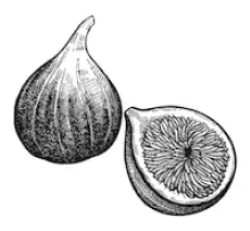
\includegraphics[width=1in,height=1.25in,clip,keepaspectratio]{figuras/author1.png}}]{Dafnh\^e Thor Castro de Martins Barros}
received the B.S. degree in Electrical Engineering. He is currently an M.Sc. candidate in Control and Automation Engineering with the Graduate Program in Control and Automation Engineering (PROPECAUT), Federal Institute of Esp\'irito Santo (IFES), Serra, Brazil. His research interests include real-time embedded systems, spaceborne computing architectures, compact thermal modeling, Model Predictive Control (MPC), and edge artificial intelligence in harsh aerospace environments.
\end{IEEEbiography}

\begin{IEEEbiography}[{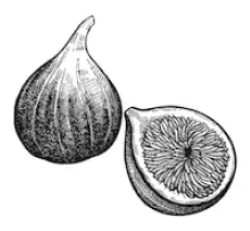
\includegraphics[width=1in,height=1.25in,clip,keepaspectratio]{figuras/author2.png}}]{Fl\'avio Barcelos Braz da Silva}
received the B.S., M.Sc., and Ph.D. degrees in Electrical Engineering. He is currently an Associate Professor with the Department of Control and Automation Engineering and a permanent faculty member of the Graduate Program in Control and Automation Engineering (PROPECAUT) at the Federal Institute of Esp\'irito Santo (IFES), Serra, Brazil. His research interests encompass robust and optimal control, space systems engineering, system identification, and embedded control.
\end{IEEEbiography}

\end{document}
